\section{Auswertung}
\label{sec:Auswertung}

\subsection{Aufnahme der Zählrohr-Charakteristik}
In Tabelle \eqref{tab:Char} ist die Zählrate $N$ in Abhängigkeit von der Spannung $U$ aufgezeigt. Im folgenden wird allerdings nur mit den nicht ausgegrauten Werten gerechnet, da nur diese zu dem Plateau der Charakteristik gehören. Das Plateau liegt wie in Abbildung \eqref{fig:Char1} zu sehen ist, zwischen 350\,V und 650\,V. Mit Hilfe einer Ausgleichsrechnung wird die Funktion des Plateaus zu
\begin{equation*}
  y = (\num{0.09 +- 0.02}) \cdot x + (\num{500 +- 10})
\end{equation*}
bestimmt. Für die Steigung in \% pro 100\,V ergibt sich
\begin{equation*}
  m = \frac{a\cdot100}{N(500\,V)} = \frac{(\num{0.09 +- 0.02})\cdot100}{545} = (\num{0.017 +- 0.004})\% \ .
\end{equation*}

\begin{table}[H]
  \centering
  \begin{tabular}{c|c|c}
    \hline
    $U$ / V & N in 10\,s & N / $\frac{1}{\text{s}}$ \\
    \hline
    \rowcolor{lightgray} 310 & 4634 & \\
    \rowcolor{lightgray} 315 & 5059 & \\
    \rowcolor{lightgray} 325 & 5223 & \\
    \hline
    \hline
    350 & 5437 & $\num{544 +- 7}$ \\
    375 & 5384 & $\num{538 +- 7}$ \\
    400 & 5368 & $\num{537 +- 7}$ \\
    450 & 5405 & $\num{541 +- 7}$ \\
    500 & 5447 & $\num{545 +- 7}$ \\
    550 & 5552 & $\num{555 +- 7}$ \\
    600 & 5485 & $\num{549 +- 7}$ \\
    625 & 5598 & $\num{560 +- 7}$ \\
    650 & 5745 & $\num{575 +- 8}$ \\
    \hline
    \hline
    \rowcolor{lightgray} 675 & 6028 & \\
    \rowcolor{lightgray} 700 & 6264 & \\
    \rowcolor{lightgray} 705 & 6443 & \\
    \hline
  \end{tabular}
  \caption{Messwerte für die Charakteristik des Zählrohrs.}
  \label{tab:Char}
\end{table}

\begin{figure}[H]
  \centering
  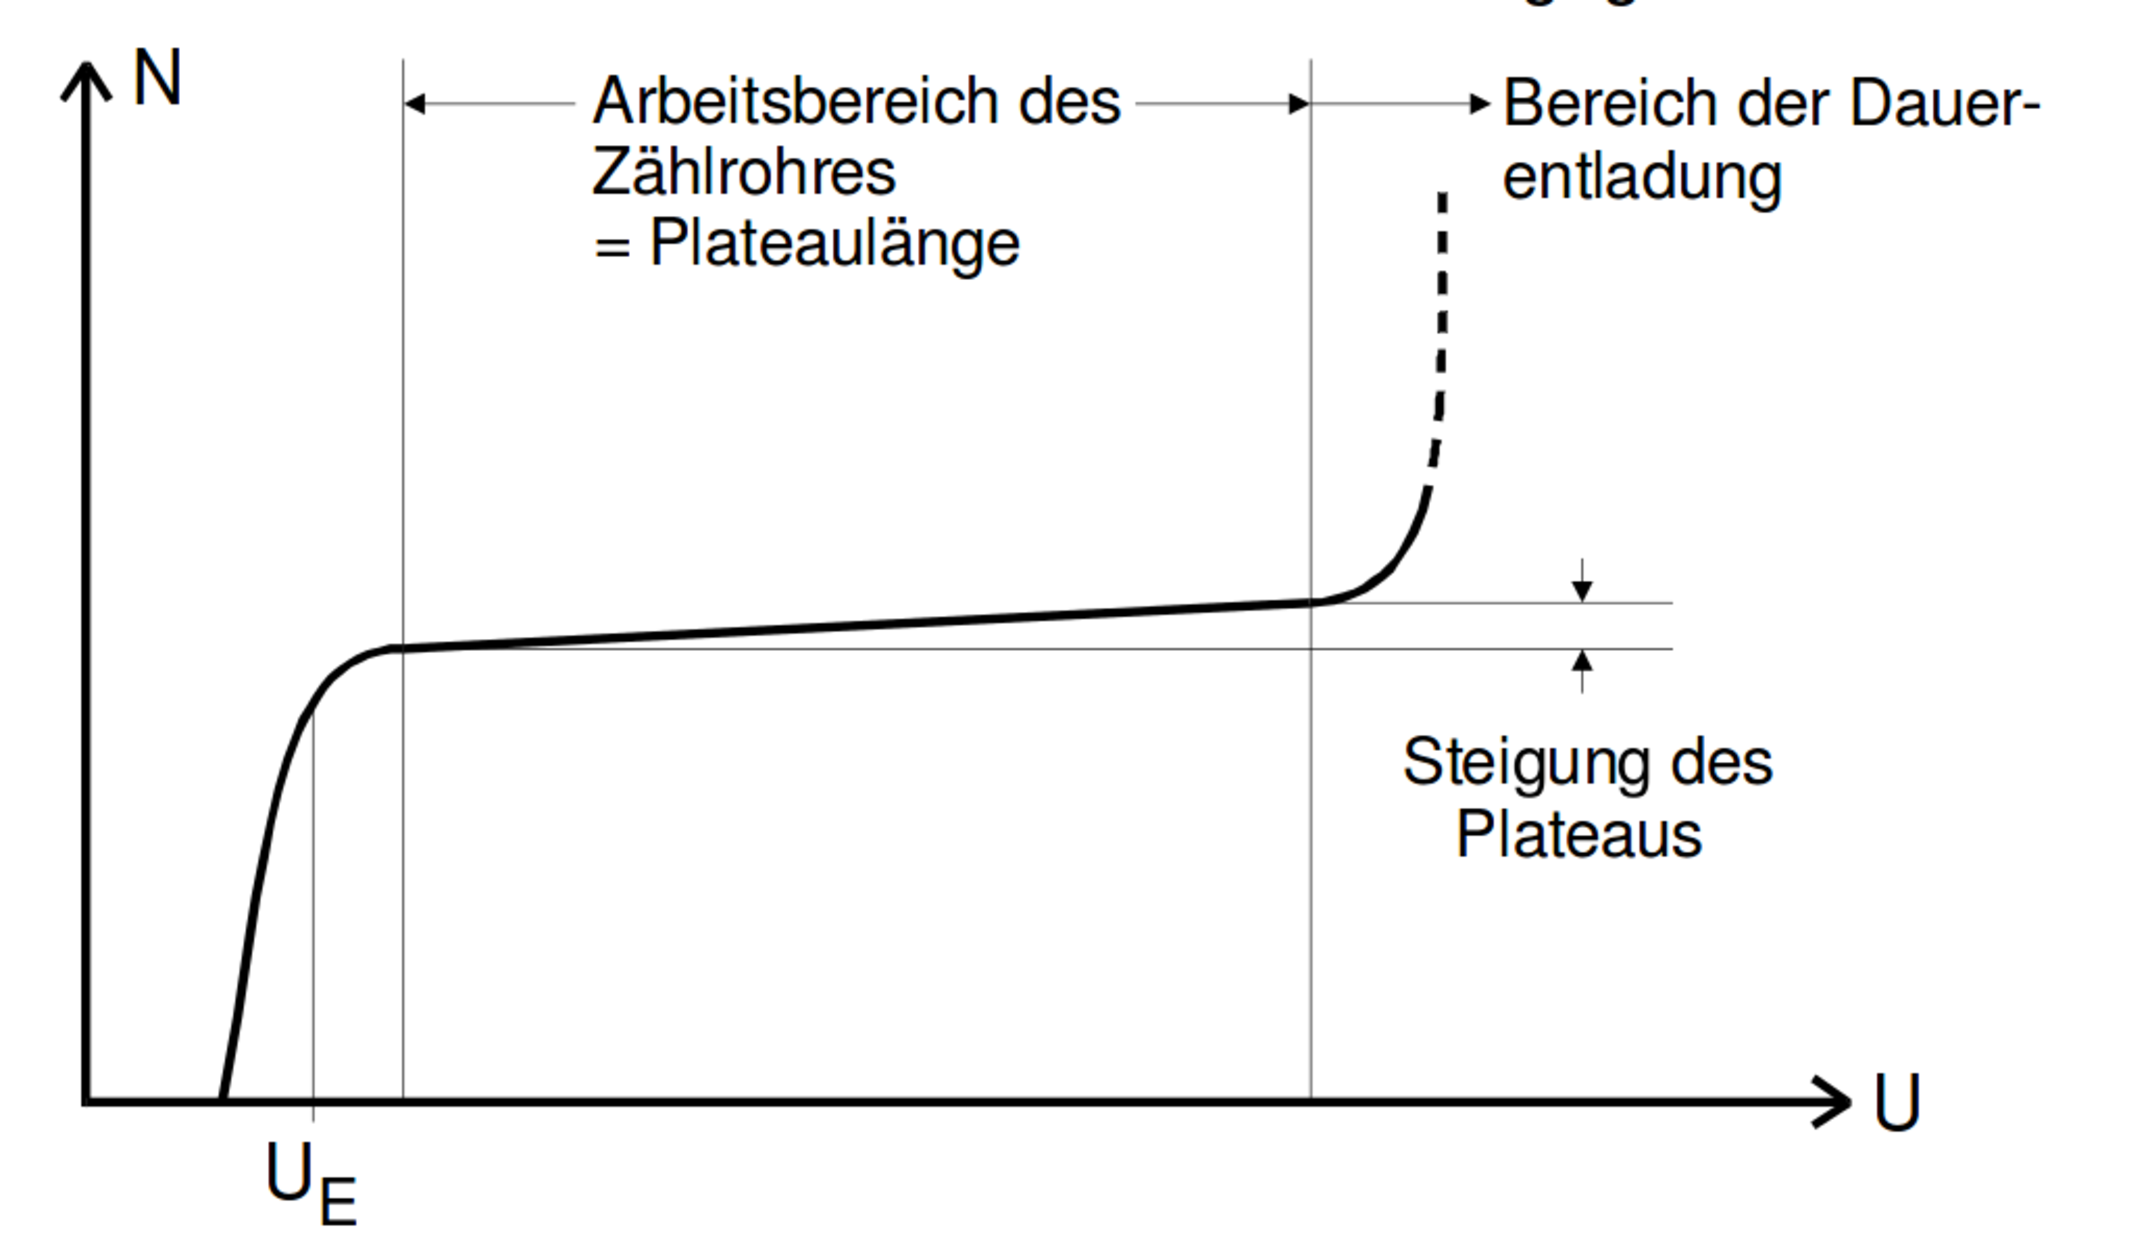
\includegraphics[height=10cm]{build/Plateau.pdf}
  \caption{Charakteristik des Zählrohres.}
  \label{fig:Char1}
\end{figure}


\subsection{Bestimmung des Abstandes von Primär- und Nachladeimpuls}
Zu Beginn dieses Versuchteils wird die Strahlintensität soweit abgesenkt das nur ein Primärmaximum für 350\,V auf dem Oszillographen zu sehen ist. Dann wird bei einer Ablenkgeschwindigkeit von 50 $\mu$s/cm der Abstand zwischen Primär- und Nachladeimpuls geschätzt. Dieser beträgt für 350\,V ($\num{220 +- 50}$)\,$\mu$s und für 700\,V ($\num{220 +- 50}$)\,$\mu$s.


\subsection{Bestimmung der Totzeit}
Die Totzeit wird auf zwei Arten gemessen. \\
Bei der ersten Methode wird die Totzeit gemäß der Abbildung \eqref{fig:tot} für 350\,V und 700\,V abgelesen.
\begin{align*}
  T_\text{350\,V} = (\num{50 +- 2})\,\mu\text{s} \\
  T_\text{700\,V} = (\num{70 +- 2})\,\mu\text{s} \\
\end{align*}
Der Mittelwert daraus beträgt
\begin{align*}
  T_\text{Osz} = (\num{60 +- 1})\,\mu\text{s}
\end{align*}
Die Messwerte für die zweite Messung sind im folgenden aufgelistet:
\begin{align*}
  N_1 = (\num{4250 +- 7})\,\frac{1}{\text{s}} \\
  N_2 = (\num{3363 +- 6})\,\frac{1}{\text{s}} \\
  N_{1+2} = (\num{7035 +- 8})\,\frac{1}{\text{s}} \\
\end{align*}
Mit Hilfe der Gleichung \eqref{eqn:T} lässt sich aus den Messwerten eine Totzeit von
\begin{align*}
  T_\text{2-Q-M} = (\num{20.2 +- 0.4})\,\mu\text{s}
\end{align*}
berechnen.


\subsection{Bestimmung der pro Teilchen im Zählrohr freigesetzten Ladungsmenge}
Mit Hilfe der Gleichung
\begin{align*}
  \overline{I} = \frac{\Delta Q\,Z}{\Delta t}
\end{align*}
und den Messwerten aus Tabelle \eqref{tab:Ladungsmenge} kann die pro Teilchen freigesetzte Ladungsmenge berechnet werden. Dabei bedeutet $\overline{I}$ den mittleren Strom, $\Delta Q$ die freigesetzte Ladungsmenge, $Z$ die Anzahl der Impulse und $\Delta t$ den Zeitraum. In Abbildung \eqref{fig:Ladungsmenge1} wird eine lineare Abhängigkeit zwischen der Spannung und der Ladungsmenge deutlich.

\begin{table}[H]
  \centering
  \begin{tabular}{c|c|c|c|c}
    \hline
    $U$ / V & $\overline{I}$ / $\mu$A & $Z$ & $\Delta Q$ / $10^{-9}$C & $\frac{\Delta Q}{e_0}\cdot10^{9}$ \\
    \hline
    310 & 0.2 & 4634 & 0.43 &  2.69 \\
    315 & 0.2 & 5059 & 0.40 &  2.47 \\
    325 & 0.4 & 5223 & 0.77 &  4.78 \\
    350 & 0.6 & 5437 & 1.10 &  6.89 \\
    375 & 0.8 & 5384 & 1.49 &  9.27 \\
    400 & 1.2 & 5368 & 2.24 & 13.95 \\
    450 & 1.8 & 5405 & 3.33 & 20.79 \\
    500 & 2.4 & 5447 & 4.41 & 27.50 \\
    550 & 3.0 & 5552 & 5.40 & 33.73 \\
    600 & 3.6 & 5485 & 6.56 & 40.97 \\
    625 & 3.7 & 5598 & 6.61 & 41.25 \\
    650 & 4.0 & 5745 & 6.96 & 43.46 \\
    675 & 4.4 & 6028 & 7.30 & 45.56 \\
    700 & 5.0 & 6264 & 7.98 & 49.82 \\
    705 & 5.0 & 6443 & 7.76 & 48.44 \\
  \end{tabular}
  \caption{Messwerte zur Bestimmung der Ladungsmenge die pro Teilchen freigesetzt wird.}
  \label{tab:Ladungsmenge}
\end{table}

\begin{figure}[H]
  \centering
  \includegraphics[height=9cm]{build/Ladungsmenge.pdf}
  \caption{Spannung gegen die Ladungsmenge aufgetragen.}
  \label{fig:Ladungsmenge1}
\end{figure}

Mit Hilfe einer linearen Ausgleichsrechnung wird der Zusammenhang zwischen der Ladungsmenge und der Spannung zu
\begin{align*}
  y = (\num{1.94 +- 0.04}) \cdot 10^{-11} \cdot x + (\num{-5.6 +- 0.2}) \cdot 10^{-9}
\end{align*}
bestimmt.
